\documentclass{report}

\input{preamble}
\input{macros}
\input{letterfonts}

\usepackage{tikz}
\usepackage{tikz-3dplot}
\usepackage{amsmath}
\usepackage{pgfplots}
\usepackage{smartdiagram}
\usesmartdiagramlibrary{additions}

\title{\Huge{CASMA 225}\\Calc 3}
\author{\huge{Giacomo Cappelletto}}
\date{4/9/24}

\begin{document}


\maketitle
\newpage
\pdfbookmark[section]{\contentsname}{toc}
\tableofcontents
\pagebreak

\chapter{Vectors}

\section{Review}

\subsection{Basics}

\dfn{Notation}{

	\begin{center}
		Drawn Vectors: $\vec{v}$ \\
		Typed Vectors: \bf{v}
	\end{center}

}

\dfn{Velocity}{

	\begin{center}
		Magnitude of the velocity: $ \abs{\vec{v}} $
		\\
		Direction of the velocity: $dir(\vec{v})$
	\end{center}
}

\dfn{Heads and Tails}{

	\begin{center}
		\begin{tikzpicture}[scale=1.5]

			% Draw the vector
			\draw[->, thick] (0,0) -- (4,2) node[midway, above] {Vector $\vec{v}$};

			% Draw the tail label
			\filldraw[black] (0,0) circle (2pt);
			\node[below left] at (0,0) {Tail};

			% Draw the head label
			\filldraw[black] (4,2) circle (2pt);
			\node[above right] at (4,2) {Head};

		\end{tikzpicture}
	\end{center}
}

\nt{Scalar is like a 1 directional vector, either positive or negative, and its magnitude is the absolute value of the scalar}

\subsection{Notation}
\dfn{Positive y axis}{

	\begin{center}
		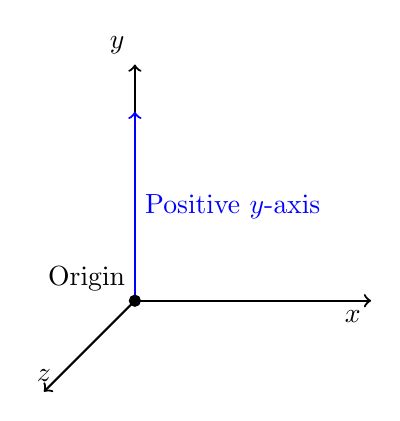
\begin{tikzpicture}[scale=2]

			% Draw the x, y, and z axes
			\draw[->, thick] (0,0,0) -- (1.5,0,0) node[anchor=north east] {$x$};
			\draw[->, thick] (0,0,0) -- (0,1.5,0) node[anchor=south east] {$y$}; % Positive y-axis
			\draw[->, thick] (0,0,0) -- (0,0,1.5) node[anchor=south] {$z$};

			% Positive y-axis with label
			\draw[->, thick, blue] (0,0,0) -- (0,1.2,0) node[midway,right] {Positive $y$-axis};

			% Draw a point at the origin
			\filldraw[black] (0,0,0) circle (1pt) node[anchor=south east] {Origin};

		\end{tikzpicture}
	\end{center}
}

\dfn{Standard Basis Vecotrs}{
	In an $n$-dimensional space $\mathbb{R}^n$, the standard basis vectors are a set of $n$ vectors where each vector has a 1 in one component and 0 in all other components. These vectors are denoted as $\mathbf{e}_i$ for $i = 1, 2, \dots, n$.

	The $i$-th standard basis vector in $\mathbb{R}^n$ is written as:

	\[
		\mathbf{e}_i =
		\begin{pmatrix}
			0                                       \\
			0                                       \\
			\vdots                                  \\
			1 \quad \text{(in the $i$-th position)} \\
			\vdots                                  \\
			0
		\end{pmatrix}
	\]

	For example, in $\mathbb{R}^3$ (three-dimensional space), the standard basis vectors are:

	\[
		\mathbf{e}_1 = \begin{pmatrix} 1 \\ 0 \\ 0 \end{pmatrix}, \quad
		\mathbf{e}_2 = \begin{pmatrix} 0 \\ 1 \\ 0 \end{pmatrix}, \quad
		\mathbf{e}_3 = \begin{pmatrix} 0 \\ 0 \\ 1 \end{pmatrix}.
	\]

	These vectors span the entire vector space $\mathbb{R}^n$, meaning any vector $\mathbf{v} \in \mathbb{R}^n$ can be written as a linear combination of the standard basis vectors:

	\[
		\mathbf{v} = v_1 \mathbf{e}_1 + v_2 \mathbf{e}_2 + \dots + v_n \mathbf{e}_n,
	\]

	where $v_1, v_2, \dots, v_n$ are the components of the vector $\mathbf{v}$.
}

\section{Operations}

\subsection{Dot Product}
\dfn{Dot (Scalar)Product Definitons}{
	The \textbf{scalar product} (or \textbf{dot product}) of two vectors \( \mathbf{a} \) and \( \mathbf{b} \) in \( \mathbb{R}^n \) is defined as:
	\[
		\mathbf{a} \cdot \mathbf{b} = a_1b_1 + a_2b_2 + \dots + a_nb_n
	\]
	In \( \mathbb{R}^3 \), for vectors \( \mathbf{a} = \begin{pmatrix} a_1 \\ a_2 \\ a_3 \end{pmatrix} \) and \( \mathbf{b} = \begin{pmatrix} b_1 \\ b_2 \\ b_3 \end{pmatrix} \), the dot product is:
	\[
		\mathbf{a} \cdot \mathbf{b} = a_1b_1 + a_2b_2 + a_3b_3
	\]
	The dot product can also be expressed in terms of the magnitudes of \( \mathbf{a} \) and \( \mathbf{b} \) and the angle \( \theta \) between them:
	\[
		\mathbf{a} \cdot \mathbf{b} = |\mathbf{a}| |\mathbf{b}| \cos \theta
	\]
	The dot product is a scalar quantity and is zero when the vectors are orthogonal (perpendicular).
	\\
	Useful to find the angle between the two vectors being dot produced together,

}

\thm{Dot Product Proof}{
	We are given the vectors $\vec{v}$ and $\vec{w}$, and we want to express the dot product in terms of their magnitudes and the angle between them.

	Start with the relationship:

	\[
		\vec{x} = \vec{v} - \vec{w}
	\]

	\begin{center}
		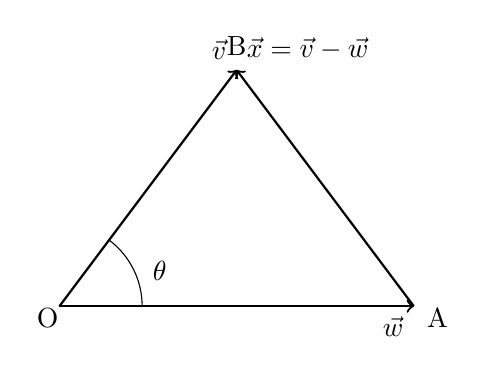
\begin{tikzpicture}[scale=1.5]
			% Draw vectors
			\draw[->, thick] (0,0) -- (3,0) node[anchor=north east] {$\vec{w}$};
			\draw[->, thick] (0,0) -- (1.5,2) node[anchor=south east] {$\vec{v}$};
			\draw[->, thick] (3,0) -- (1.5,2) node[anchor=south west] {$\vec{x} = \vec{v} - \vec{w}$};

			% Label the angle theta
			\draw (0.7,0) arc[start angle=0,end angle=53,radius=0.7];
			\node at (0.85,0.3) {$\theta$};

			% Draw point labels
			\node at (-0.1,-0.1) {O};
			\node at (3.2,-0.1) {A};
			\node at (1.5,2.2) {B};
		\end{tikzpicture}
	\end{center}

	The above diagram illustrates the vectors $\vec{v}$, $\vec{w}$, and their difference $\vec{x} = \vec{v} - \vec{w}$, forming a triangle. The angle $\theta$ is between $\vec{v}$ and $\vec{w}$.

	The magnitude squared of $\vec{x}$ is:

	\[
		|\vec{x}|^2 = |\vec{v}|^2 + |\vec{w}|^2 - 2|\vec{v}||\vec{w}|\cos\theta
	\]

	This is the expansion of the law of cosines.

	Now, from the equation:

	\[
		|\vec{x}|^2 = \sqrt[2]{\left( (v_x - w_x)^2 + (v_y - w_y)^2 \right)}^2
	\]

	We conclude:

	\[
		|\vec{x}|^2 = |\vec{v}|^2 + |\vec{w}|^2 - 2 (\vec{v} \cdot \vec{w})
	\]

	Thus, we can express the dot product $\vec{v} \cdot \vec{w}$ as:

	\[
		\vec{v} \cdot \vec{w} = |\vec{v}||\vec{w}|\cos\theta
	\]
}

\subsection{Applications}

\nt{
	The dot product of two vectors $\vec{v} \cdot \vec{w}$ can take different values, leading to various interpretations of the relationship between the vectors. Below is a table describing some key cases:

	\begin{center}
		\begin{tabular}{|c|c|c|}
			\hline
			\textbf{Dot Product Value}                    & \textbf{Interpretation}         & \textbf{Relationship Between Vectors}                                                         \\
			\hline
			$\vec{v} \cdot \vec{w} = 0$                   & $\cos\theta = 0$                & Vectors are \textbf{perpendicular} (orthogonal), $\theta = 90^\circ$                          \\
			\hline
			$\vec{v} \cdot \vec{w} > 0$                   & $0 < \theta < 90^\circ$         & Vectors form an \textbf{acute angle}, pointing in the same general direction                  \\
			\hline
			$\vec{v} \cdot \vec{w} < 0$                   & $90^\circ < \theta < 180^\circ$ & Vectors form an \textbf{obtuse angle}, pointing in opposite general directions                \\
			\hline
			$\vec{v} \cdot \vec{w} = |\vec{v}||\vec{w}|$  & $\cos\theta = 1$                & Vectors are \textbf{parallel} and point in the \textbf{same direction}, $\theta = 0^\circ$    \\
			\hline
			$\vec{v} \cdot \vec{w} = -|\vec{v}||\vec{w}|$ & $\cos\theta = -1$               & Vectors are \textbf{parallel} but point in \textbf{opposite directions}, $\theta = 180^\circ$ \\
			\hline
		\end{tabular}
	\end{center}
}

\dfn{Vector Product (Cross Product)}{
	The \textbf{vector product} (or \textbf{cross product}) of two vectors \( \mathbf{a} \) and \( \mathbf{b} \) in \( \mathbb{R}^3 \) is a vector \( \mathbf{c} \) that is perpendicular to both \( \mathbf{a} \) and \( \mathbf{b} \), and its magnitude is given by:
	\[
		|\mathbf{c}| = |\mathbf{a} \times \mathbf{b}| = |\mathbf{a}| |\mathbf{b}| \sin \theta
	\]
	where \( \theta \) is the angle between \( \mathbf{a} \) and \( \mathbf{b} \). The cross product is calculated as:
	\[
		\mathbf{a} \times \mathbf{b} = \begin{vmatrix}
			\hat{i} & \hat{j} & \hat{k} \\
			a_1     & a_2     & a_3     \\
			b_1     & b_2     & b_3
		\end{vmatrix} = (a_2b_3 - a_3b_2)\hat{i} - (a_1b_3 - a_3b_1)\hat{j} + (a_1b_2 - a_2b_1)\hat{k}
	\]
	The result of a cross product is a vector perpendicular to the plane formed by \( \mathbf{a} \) and \( \mathbf{b} \), with a direction given by the right-hand rule.
}

\dfn{Vector Projections} {
% Vector projection diagram

\begin{center}
	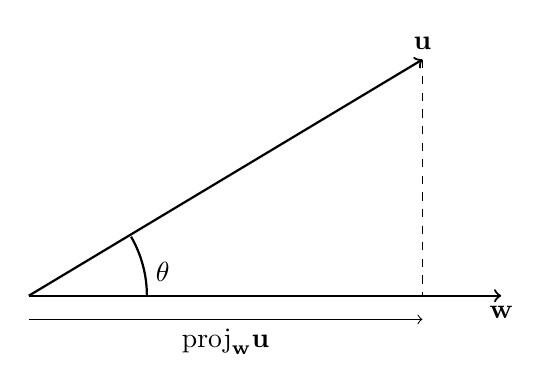
\begin{tikzpicture}
		% Draw vector w
		\draw[->, thick] (0,0) -- (6,0) node[anchor=north] {$\mathbf{w}$};

		% Draw vector u
		\draw[->, thick] (0,0) -- (5,3) node[anchor=south] {$\mathbf{u}$};

		% Projection line
		\draw[dashed] (5,3) -- (5,0) node[anchor=north] {};

		% Angle theta
		\draw[thick] (1.5,0) arc (0:30:1.5);
		\node at (1.7,0.3) {$\theta$};

		% Label projection of u on w
		\draw[->] (0,-0.3) -- (5,-0.3) node[midway,below] {$\text{proj}_{\mathbf{w}}\mathbf{u}$};
	\end{tikzpicture}
\end{center}

\[
	\text{scal}_{\mathbf{w}}\mathbf{u} = |\mathbf{u}| \cdot \cos\theta = \frac{\mathbf{w} \cdot \mathbf{u}}{|\mathbf{w}|}
\]

\[
	\text{proj}_{\mathbf{w}} \mathbf{u} = |\mathbf{u}| \cos \theta \left( \frac{\mathbf{w}}{|\mathbf{w}|} \right)
\]

\[
	\text{proj}_{\mathbf{w}} \mathbf{u} = \left( \frac{\mathbf{w} \cdot \mathbf{u}}{\mathbf{w} \cdot \mathbf{w}} \right) \mathbf{w}
\]
}

\section{Matrix Determinants}

\dfn{Matrix Representation}{
	A matrix is a collection of numbers arranged in a grid format, where each element is positioned based on its row and column. A general $m \times n$ matrix is written as:
	\[
		M =
		\begin{pmatrix}
			a_{11} & a_{12} & \cdots & a_{1n} \\
			a_{21} & a_{22} & \cdots & a_{2n} \\
			\vdots & \vdots & \ddots & \vdots \\
			a_{m1} & a_{m2} & \cdots & a_{mn} \\
		\end{pmatrix}
	\]
	For example, a $2 \times 2$ matrix is given by:
	\[
		M = \begin{pmatrix} a & b \\ c & d \end{pmatrix}
	\]
	A $3 \times 3$ matrix is:
	\[
		M = \begin{pmatrix} a & b & c \\ d & e & f \\ g & h & i \end{pmatrix}
	\]
	Matrices can be considered as a collection of vectors where each row or column can represent a vector.
}

\nt{\textbf{Vector Representation} \\
	A matrix can also be viewed as a collection of vectors. For instance, a $3 \times 3$ matrix can be interpreted as:
	\[
		M = \begin{pmatrix}
			\vec{v_1} = \langle a, b, c \rangle \\
			\vec{v_2} = \langle d, e, f \rangle \\
			\vec{v_3} = \langle g, h, i \rangle
		\end{pmatrix}
	\]
	where each row (or column) is treated as a vector in space.
}

\dfn{Determinant of a $2 \times 2$ Matrix}{
	The determinant of a $2 \times 2$ matrix is given by:
	\[
		\text{det}(M) = \det\begin{pmatrix} a & b \\ c & d \end{pmatrix} = ad - bc
	\]
	The determinant represents the signed area of the parallelogram formed by the vectors corresponding to the rows (or columns) of the matrix.


	\begin{center}
		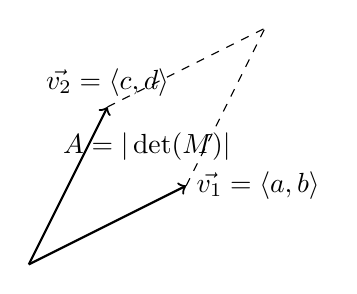
\begin{tikzpicture}
			% Define the vectors
			\draw[->, thick] (0,0) -- (2,1) node[right] {$\vec{v_1} = \langle a, b \rangle$};
			\draw[->, thick] (0,0) -- (1,2) node[above] {$\vec{v_2} = \langle c, d \rangle$};

			% Draw the parallelogram
			\draw[dashed] (2,1) -- (3,3);
			\draw[dashed] (1,2) -- (3,3);

			% Label the area
			\node at (1.5, 1.5) {$A = |\det(M)|$};
		\end{tikzpicture}
	\end{center}

}

\nt{\textbf{Geometric Interpretation} \\
	For a $2 \times 2$ matrix, the determinant represents the area $A$ of the parallelogram formed by the two vectors $\vec{v_1} = \langle a, b \rangle$ and $\vec{v_2} = \langle c, d \rangle$. The magnitude of the determinant gives the area of this parallelogram, and the sign of the determinant indicates the orientation (whether the vectors are ordered clockwise or counterclockwise).
}

\dfn{Determinant of a $3 \times 3$ Matrix}{
	The determinant of a $3 \times 3$ matrix is calculated as:
	\[
		\text{det}(M) = \det \begin{pmatrix}
			a & b & c \\
			d & e & f \\
			g & h & i
		\end{pmatrix}
		= a \det \begin{pmatrix} e & f \\ h & i \end{pmatrix}
		- b \det \begin{pmatrix} d & f \\ g & i \end{pmatrix}
		+ c \det \begin{pmatrix} d & e \\ g & h \end{pmatrix}
	\]
	The determinant represents the signed volume of the parallelepiped formed by the three vectors corresponding to the rows (or columns) of the matrix.
	\begin{center}
		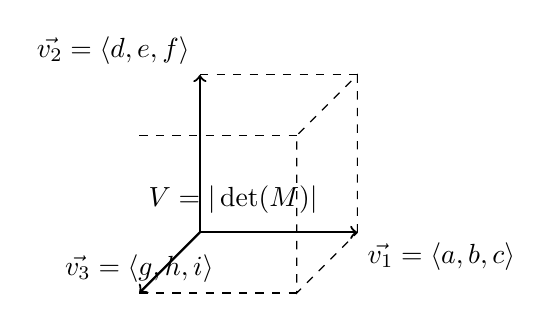
\begin{tikzpicture}
			% Define the 3D vectors
			\draw[->, thick] (0,0,0) -- (2,0,0) node[below right] {$\vec{v_1} = \langle a, b, c \rangle$};
			\draw[->, thick] (0,0,0) -- (0,2,0) node[above left] {$\vec{v_2} = \langle d, e, f \rangle$};
			\draw[->, thick] (0,0,0) -- (0,0,2) node[above] {$\vec{v_3} = \langle g, h, i \rangle$};

			% Draw the parallelepiped
			\draw[dashed] (2,0,0) -- (2,2,0) -- (2,2,2) -- (2,0,2) -- cycle;
			\draw[dashed] (0,2,0) -- (2,2,0);
			\draw[dashed] (0,0,2) -- (2,0,2);
			\draw[dashed] (0,2,2) -- (2,2,2);

			% Label the volume
			\node at (1,1,1.5) {$V = |\det(M)|$};
		\end{tikzpicture}
	\end{center}

}

\nt{\textbf{Geometric Interpretation for $3 \times 3$} \\
	In the $3 \times 3$ case, the determinant represents the volume $V$ of the parallelepiped formed by three vectors $\vec{v_1}, \vec{v_2}, \vec{v_3}$, and the sign indicates whether the orientation is right-handed or left-handed. The magnitude gives the volume.
}

\section{Matrix multiplication with 2D Vectors}

\dfn{Vector Matrix Multiplication}{

	\[
		M = \begin{pmatrix} a_{11} & a_{12} \\ a_{21} & a_{22} \end{pmatrix}, \quad
		V = \begin{pmatrix} V_1 \\ V_2 \end{pmatrix}
	\]

	\[
		\hat{\mathbf{j}}M = \langle a_{11}V_1 + a_{12}V_2, a_{21}V_1 + a_{22}V_2 \rangle
	\]

	Given:
	\[
		\hat{i} = \langle 1, 0 \rangle \quad \hat{j} = \langle 0, 1 \rangle
	\]

	We can compute:
	\[
		iM = \langle a_{11}, a_{12} \rangle = a_1
	\]
	\[
		jM = \langle a_{21}, a_{22} \rangle = a_2
	\]

	Where:
	\[
		\mathbf{V} = V_1 \hat{i} + V_2 \hat{j}
	\]
	\[
		\hat{\mathbf{V}}M = \left( V_1 \hat{i} + V_2 \hat{j} \right) M
	\]
	\[
		= V_1 \hat{i} M + V_2 \hat{j} M
	\]
	\[
		= V_1 \mathbf{a}_1 + V_2 \mathbf{a}_2
	\]

}

\nt{
	\centering
	\includegraphics[width=0.5\textwidth]{graphicalvm.png} % Adjust the width as needed
	\par\vspace{1em} % Adds a small space after the image
}

\subsection{Effect on Area}

\dfn{$2D$}{
The original point \( (1,1) \) is transformed by the matrix \( M \). This transformation impacts the area and orientation as follows:

\[
	M = \begin{pmatrix} a_{11} & a_{12} \\ a_{21} & a_{22} \end{pmatrix}
\]

The area after transformation is given by the determinant of the matrix:

\[
	\text{Area} = \det(M)
\]
Where the determinant is calculated as:
\[
	\det(M) = a_{11}a_{22} - a_{12}a_{21}
\]

The determinant also determines the orientation:
\[
	\det(M) = \begin{cases}
		A  & \text{if } a_1 \text{ to } a_2 \text{ is counterclockwise} \\
		-A & \text{otherwise}
	\end{cases}
\]

In the example, the original vectors \( a_1 \) and \( a_2 \) form an area, and the determinant will tell us if the vectors are oriented in a clockwise or counterclockwise fashion.

If the determinant is negative, the orientation is clockwise, as illustrated:

\[
	\det \left( \begin{pmatrix} a_1 & a_2 \end{pmatrix} \right) < 0
\]

Thus, in this case, the transformation results in a clockwise orientation.
}

\section{Matrix multiplication with 3D Vectors}

\dfn{$3D$}{
	The matrix \( M \) for a 3D transformation is given as:

	\[
		M = \begin{pmatrix}
			a_{11} & a_{12} & a_{13} \\
			a_{21} & a_{22} & a_{23} \\
			a_{31} & a_{32} & a_{33}
		\end{pmatrix}
		\quad
		\text{where} \quad
		\vec{V} = \langle V_1, V_2, V_3 \rangle
	\]

	The transformation of vector \( \vec{V} \) under matrix \( M \) is:

	\[
		\hat{\vec{V}} M = \langle (a_{11} V_1 + a_{12} V_2 + a_{13} V_3), (a_{21} V_1 + a_{22} V_2 + a_{23} V_3), (a_{31} V_1 + a_{32} V_2 + a_{33} V_3) \rangle
	\]

	This can be written in terms of the basis vectors as:
	\[
		\left( V_1 \hat{i} + V_2 \hat{j} + V_3 \hat{k} \right) M = V_1 \vec{a}_1 + V_2 \vec{a}_2 + V_3 \vec{a}_3
	\]

}

\dfn{orientation and Volume}{
	- If the determinant of matrix \( M \) is negative, the system is **left-handed**, i.e.,
	\[
		\det(M) = -V
	\]
	- The determinant of the matrix \( M \) gives the **volume** of the parallelepiped spanned by the vectors \( a_1, a_2, a_3 \):

	\[
		\det(M) = \text{Volume}(V)
	\]

	The volume \( V \) is given by:
	\[
		V = \begin{cases}
			+V & \text{if } \vec{a}_1, \vec{a}_2, \vec{a}_3 \text{ are right-handed (RHS)} \\
			-V & \text{otherwise (left-handed)}
		\end{cases}
	\]
}

\section{Cross Product and Volumes}

\dfn{Cross Product and Volumes}{
	The volume of a parallelepiped defined by three vectors \( \vec{u}, \vec{v}, \vec{w} \) is given by:
	\[
		\text{V} = \vec{u} \cdot (\vec{v} \times \vec{w})
	\]
}

\subsection{Link to Matrix Determinants}

\dfn{Cross Product and Matrix Determinants}{
	\textbf{Since:}
	\[
		\vec{u} \cdot (\vec{v} \times \vec{w}) = \det \begin{pmatrix} \vec{u} & \vec{v} & \vec{w} \end{pmatrix}
	\]

	\[
		\det \begin{pmatrix}
			u_1 & u_2 & u_3 \\
			v_1 & v_2 & v_3 \\
			w_1 & w_2 & w_3
		\end{pmatrix}
		=
		u_1 \det \begin{pmatrix} v_2 & v_3 \\ w_2 & w_3 \end{pmatrix}
		- u_2 \det \begin{pmatrix} v_1 & v_3 \\ w_1 & w_3 \end{pmatrix}
		+ u_3 \det \begin{pmatrix} v_1 & v_2 \\ w_1 & w_2 \end{pmatrix}
	\]

	\[
		= \vec{u} \cdot
		\left(
		\hat{i} \begin{vmatrix} v_2 & v_3 \\ w_2 & w_3 \end{vmatrix}
		- \hat{j} \begin{vmatrix} v_1 & v_3 \\ w_1 & w_3 \end{vmatrix}
		+ \hat{k} \begin{vmatrix} v_1 & v_2 \\ w_1 & w_2 \end{vmatrix}
		\right)
	\]

	\[
		= \vec{u} \cdot \det \begin{pmatrix} \hat{i} & \hat{j} & \hat{k} \\ v_1 & v_2 & v_3 \\ w_1 & w_2 & w_3 \end{pmatrix}
	\]

	\[
		= \vec{u} \cdot (\vec{v} \times \vec{w})
	\]

	\textbf{Therefore:}

	\[
		\vec{v} \times \vec{w} = \det \begin{pmatrix} \hat{i} & \hat{j} & \hat{k} \\ v_1 & v_2 & v_3 \\ w_1 & w_2 & w_3 \end{pmatrix}
	\]
}

\section {Cross Product Polynomial Multiplication}

\dfn{Properties}{

	\[
		\hat{i} \times \hat{j} = \hat{k}, \quad \hat{j} \times \hat{k} = \hat{i}, \quad \hat{k} \times \hat{i} = \hat{j}
	\]

	\[
		\hat{j} \times \hat{i} = -\hat{k}, \quad \hat{i} \times \hat{i} = \hat{j} \times \hat{j} = \hat{k} \times \hat{k} = 0
	\]
}

\ex{Example: Cross Product}{
	Let \( \vec{v} = 2\hat{i} - \hat{j} - 3\hat{k} \) and \( \vec{w} = \hat{i} + \hat{j} + \hat{k} \). The cross product \( \vec{v} \times \vec{w} \) is computed as:

	\[
		\vec{v} \times \vec{w} = \left( 2\hat{i} - \hat{j} - 3\hat{k} \right) \times \left( \hat{i} + \hat{j} + \hat{k} \right)
	\]

	Expanding the cross product term by term:

	\[
		= 2\hat{i} \times \hat{i} + 2\hat{i} \times \hat{j} + 2\hat{i} \times \hat{k}
		- \hat{j} \times \hat{i} - \hat{j} \times \hat{j} - \hat{j} \times \hat{k}
		- 3\hat{k} \times \hat{i} - 3\hat{k} \times \hat{j} - 3\hat{k} \times \hat{k}
	\]

	Using the cross product identities:

	\[
		= 0 + 2\hat{k} + 2(-\hat{j})
		- (-\hat{k}) + 0 - \hat{i}
		- 3\hat{j} + 3\hat{i} + 0
	\]

	Combining like terms:

	\[
		= (3\hat{i} - \hat{i}) + (-2\hat{j} - 3\hat{j}) + (2\hat{k} + \hat{k})
	\]

	\[
		= 2\hat{i} - 5\hat{j} + 3\hat{k}
	\]

	Thus, the final result is:

	\[
		\vec{v} \times \vec{w} = 2\hat{i} - 5\hat{j} + 3\hat{k}
	\]
}

\section{Torque}

\dfn{Torque and Angular Momentum}{
	Continue with Torque
}


\end{document}